\documentclass{article}

\usepackage{kafkanotes}

\title{Lecture Notes on Quantum Mechanics}
\author{Daniel David Torres Amaris}

\begin{document}

\begin{titlepage}
\thispagestyle{empty}
\maketitle

\begin{abstract}
Lecture notes on Quantum Mechanics for 2024-2 course taught at the Universidad de Pamplona. This document consists mainly of a compilation of my notes after studying the books of Sakurai and Zettili along with the exercises and examples that I used along the course.
\end{abstract}

\tableofcontents
\end{titlepage}

\newgeometry{top=20mm,bottom=25mm,right=80mm,left=20mm}


\section{Introduction}
Before quantum mechanics, everything was explained in terms of particles and waves, separated worlds whose interaction was described by the Lorentz force or by thermodynamics. Only relativistic and microscopic systems were out of the reach of Newtonian physics. Atomic stability, atomic spectra, the photoelectric effect and black body radiation where the final problems of physics. Quantum mechanics has its origins on the attempt to explain the differences observed between the emission spectra of gases and a black body. The first showed a discrete behavior while latter turned out continuous. 
\begin{marginfigure}%
  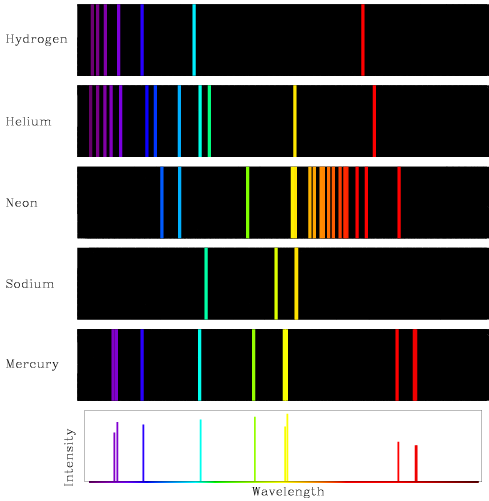
\includegraphics[width=\linewidth]{figures/lec19_elements}
  \caption{Discrete spectra for various gases.}
  \label{fig:gasesspect}
\end{marginfigure}
A black body (see fig. \ref{fig:blackbodyimg}) consists of a system emits the same amount of energy that it absorbs; a real life realization of a black body can be achieved by metallic box with reflecting walls and one hole. In such a system, the hole behaves as a black body, absorbing all the wavelengths and emitting all of them after multiple reflection over the inner part of the box. Thus, a black body is a perfect absorber and a perfect emitter.
\begin{marginfigure}%
  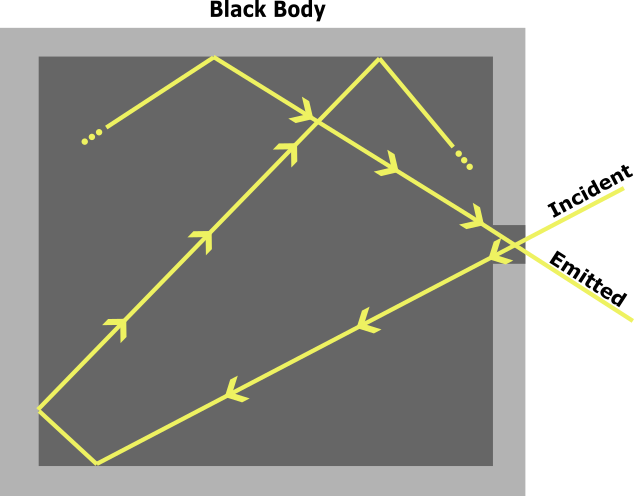
\includegraphics[width=\linewidth]{figures/blackbodyimg}
  \caption{Physical realization of a black body.}
  \label{fig:blackbodyimg}
\end{marginfigure}
Besides this notorious differences, further difficulties arose from the very description of the black body radiation. Experimental measurements performed on a variety of black bodies made out of different materials showed energy distributions with zero radiance for the 0 nm wavelength, then increasing until a maximum after which the radiance decreases monotonically until it becomes vanishingly small for large wavelengths. The solid curve in fig. \ref{fig:blackbodyrad} depicts the mentioned behavior.
\begin{figure}%
  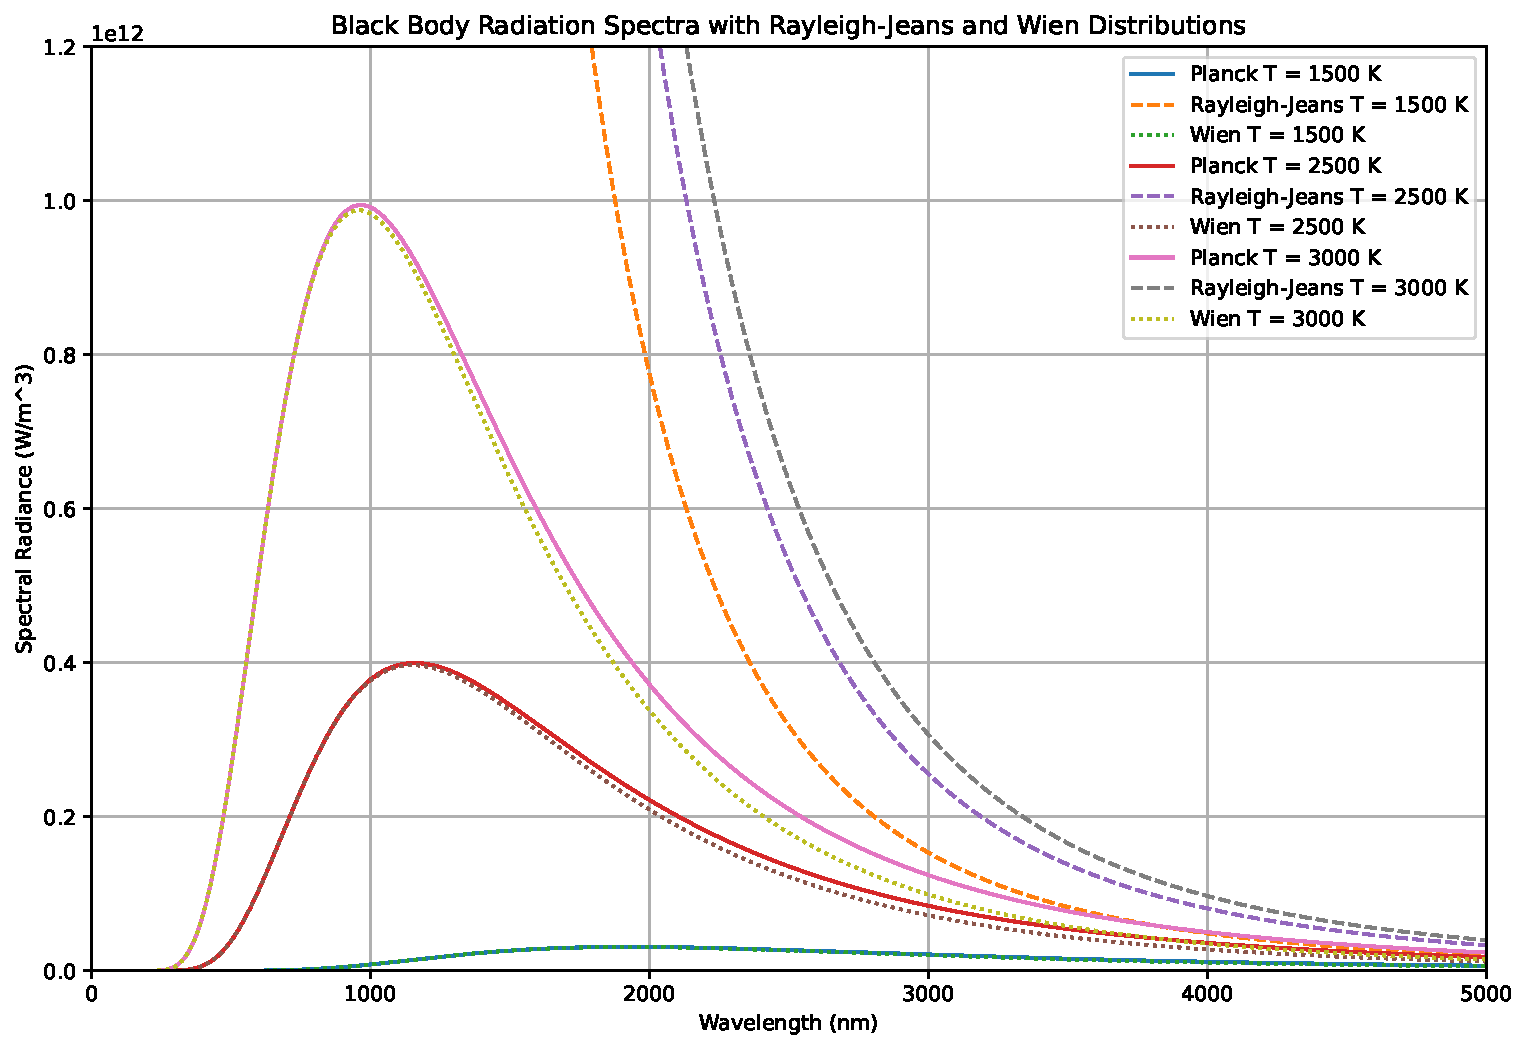
\includegraphics[width=\linewidth]{figures/blackbody}
  \caption{Black body radiance distribution.}
  \label{fig:blackbodyrad}
\end{figure}
Attempts to describe the observed behavior where made by Wien and by Rayleigh (see doted and dashed plots respectively in fig. \ref{fig:blackbodyrad}). The Wien's law, derived the spectral radiance $u(\lambda,T)$ from the thermodynamic point of view, achieves a good approximation for small wavelengths and discrepancies for high wavelengths, according to the following equation
\begin{equation}
  u(\lambda, T) = \frac{2hc^2}{\lambda^5} e^{-\frac{hc}{\lambda k_\text{B} T}},
\end{equation}
where $\lambda$ is the wavelength, T is the temperature in Kelvin, $h$, $k_B$ and $c$ are the Planck's, Boltzmann's and the speed of light constants.
The Rayleigh-Jeans distribution, derived from statistics considering the cavity full of standing waves at equilibrium and using the equipartition theorem, arrived to a clear impossibility where the system can have an infinite total energy and infinite radiance is allowed for small wavelengths! 
\begin{equation}
  u(\lambda,T) = \frac{2ck_\text{B}T}{\lambda^4}.
\end{equation}
Planck in an attempt to improve the fitting of the Wien's distribution used a similar procedure than Rayleigh's. Thus, starting from the average energy for the harmonic oscillators inside the cavity
\begin{equation}\label{eq:equipart}
  <E> = \frac{\int_0^\infty E e^{-E/k_B T}dE}{\int_0^\infty e^{-E/k_B T}dE},
\end{equation}
but postulating discrete emitting harmonic oscillators allowed only to emit energy in multiples of $h\nu$,
\begin{equation}
  E = nh\nu, n=0,1,2,...
\end{equation}
he was able to change the integral in eq. \ref{eq:equipart} for a summation as follows
\begin{equation}\label{eq:planckequipart}
  <E> = \frac{\sum_{n=0}^\infty nh\nu e^{-nh\nu/k_B T}}{\sum_{n=0}^\infty e^{-nh\nu/k_B T}} = \frac{h\nu}{e^{\frac{h\nu}{k_B T}}-1}.
\end{equation}
Multiplying eq \ref{eq:planckequipart} by the number of modes allowed inside the cavity, we have:
\begin{equation}\label{eq:planckrad}
  u(\nu,T) = \frac{8\pi\nu^2}{c^3} \frac{h\nu}{e^{\frac{h\nu}{k_B T}}-1}.
\end{equation}
Notice that you can find the Wien's and Rayleigh's distributions in terms of the frequency by using the substitution $\lambda^{-1}=\frac{\nu}{c}$. This calculation is left as an exercise for the student.
Direct integration of eq. \ref{eq:planckrad} over all the whole spectrum gives
\begin{equation}\label{eq:plancktotal}
  E_{Total} = \int_{0}^{\infty}u(\nu,T)d\nu = \frac{8\pi h}{c^3} \int_0 ^{\infty} \frac{\nu^3}{e^{\frac{h\nu}{k_B T}}-1}=\frac{8\pi^5k_B ^4}{15h^3 c^3}T^4=\frac{4}{c}\sigma T^4,
\end{equation}
where $\sigma$ is the Stefan-Boltzmann constant. In eq. \ref{eq:plancktotal} the total energy is not longer infinite but always depending on the temperature as expected. Furthermore, eq. \ref{eq:planckrad} fitted perfectly with the experimental data. Thus, Planck's distribution for black body radiation solved both the ultraviolet catastrophe and worked seamlessly both in the low and high frequency ranges. All thanks to the discretization imposed over the energy emitted by the oscillators. 
In what follows, we are going to see how this idea was taken by other scientists to solve the remaining problems.
\subsection{Exercises}
\begin{itemize}
  \item Calculate the number of modes allowed inside a cubic cavity of volume v=$a^3$ 
  \item Find the expressions for the Wien's and Rayleigh-Jeans' distributions in terms of the frequency
  \item 
\end{itemize}

\section{Compton effect}
The compton effect consist of a shift in wavelength observed for x-ray or $\gamma$-ray photons that scatters away from electrons initially at rest. This interaction provides evidence for the particle behavior of the light; here, the photon is not absorbed, instead, it collides with the electron. After colliding, the electron recoils making the photon lose some of its energy and momentum which is gained to the electron. Therefore, the wavelength of the photon is increased. In fig. \ref{fig:compton} an illustration of process is shown
\begin{marginfigure}%
  \begin{tikzpicture}
    \node[anchor=south west,inner sep=0] at (0,0) {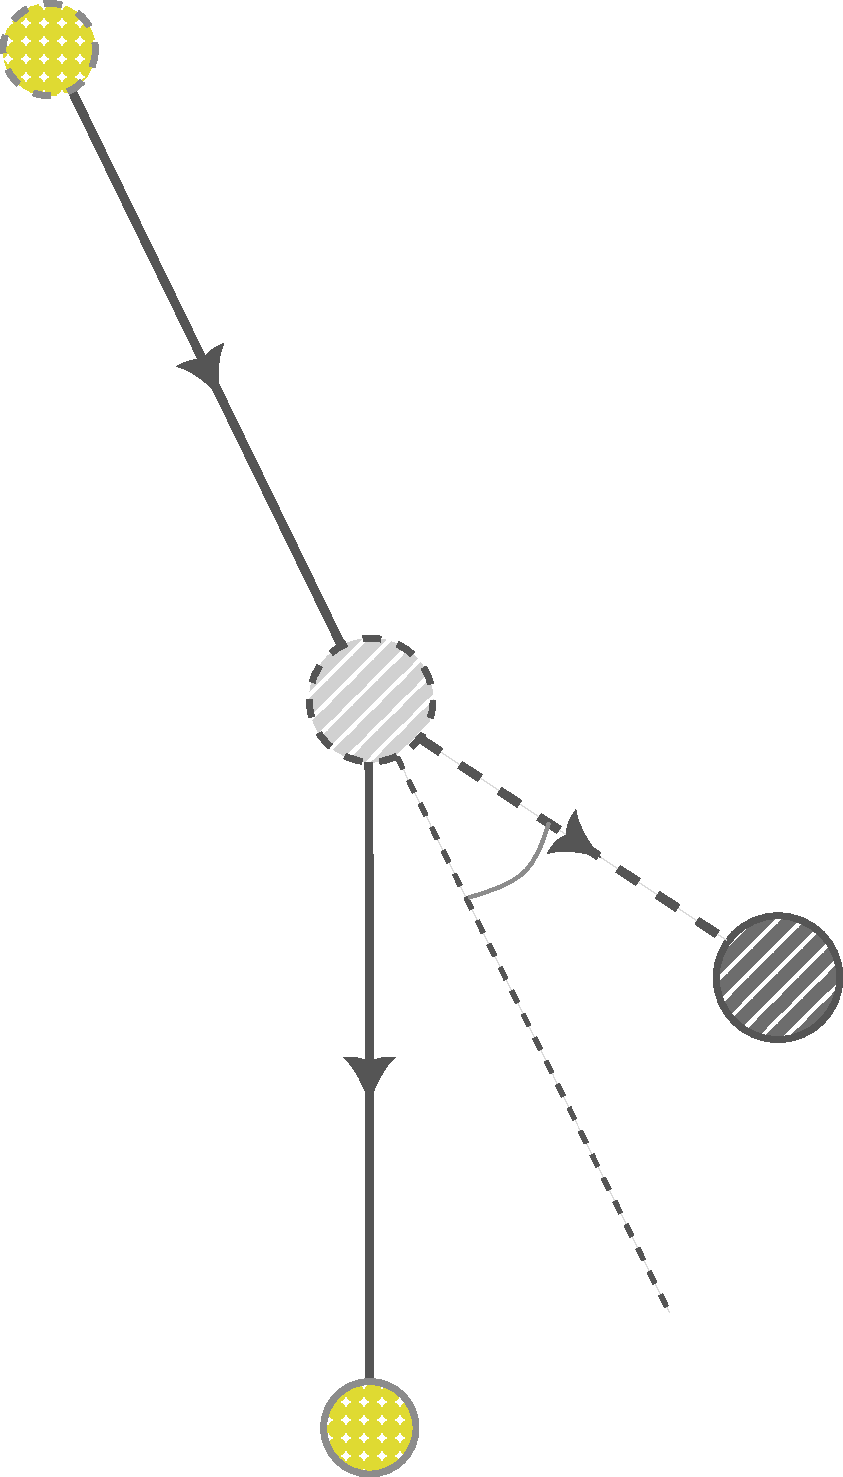
\includegraphics[width=\textwidth]{figures/compton.pdf}};
    \node at (2.3,10.2) {$\gamma: $ $E=h\nu$, $\vec{p}=\frac{h\nu}{c}$};
    \node at (4.5,0.4) {\resizebox{0.45\textwidth}{!}{$\gamma': $ $E'=h\nu'$, $\vec{p'}=\frac{h\nu'}{c}$}};
    \node at (4.5,5.6) {\resizebox{0.43\textwidth}{!}{$e^-:$ $E_e =m_ec^2$, $\vec{p}_e=0$}};
    \node at (5.1,2.7) {\resizebox{0.26\textwidth}{!}{${e^-}':$ $E'_e$, $\vec{p'}_e$}};
    \node at (3.5,4.5) {$\theta$};
  \end{tikzpicture}
  \caption{Compton effect: a photon scatters away from an electron, suffering a change in its wavelength along the process.}
  \label{fig:compton}
\end{marginfigure}
Momentum conservation law can be written as
\begin{equation}\label{eq:momentumconserv}
  \vec{p}+\vec{p}_e=\vec{p'}+\vec{p'}_e,
\end{equation}
but, the electron is initially at rest
\begin{equation}\label{eq:momentumconserv1}
  \vec{p}=\vec{p'}+\vec{p'}_e.  
\end{equation}
Thus, the explicit equation for the electron's momentum after the collision is
\begin{equation}\label{eq:momentumconserv2}
  \vec{p'}_e=\vec{p}-\vec{p'}\rightarrow{p'}^2_e=p^2+{p'}^2-2pp'\cos\theta,
\end{equation}
which, in terms of the frequency results as
\begin{equation}\label{eq:momentumconserv3}
  {p'}^2_e=\left(\frac{h\nu}{c}\right)^2+\left(\frac{h\nu'}{c}\right)^2-2\left(\frac{h\nu}{c}\right)\left(\frac{h\nu'}{c}\right)\cos\theta
\end{equation}
or
\begin{equation}\label{eq:momentumconserv4}
  {p'}^2_e=\frac{h^2}{c^2}\left(\nu^2+\nu'^2-2\nu\nu'\cos\theta\right).
\end{equation}

On the other hand, the energy conservation law demands 
\begin{equation}\label{eq:energyconserv}
  E+E_e=E'+E'_e.
\end{equation}
The energy momentum relation for the electron
\begin{equation}\label{eq:energyconserv1}
  E_e^2 = (p_e \textrm c)^2 + \left(m_e \textrm c^2\right)^2=h\sqrt{\nu^2+\nu'^2-2\nu\nu'\cos\theta +\frac{m_e^2c^4}{h^2}}
\end{equation}
in combination with the momentum of the electron after the collision (eq. \ref{eq:momentumconserv4}) results in 
\begin{equation}\label{eq:energyconserv2}
  h\nu + m_ec^2 = h\nu' + h\sqrt{\nu^2+\nu'^2-2\nu\nu'\cos\theta +\frac{m_e^2c^4}{h^2}}.
\end{equation}
which can be rewritten as
\begin{equation}\label{eq:energyconserv3}
  \nu - \nu' + \frac{m_ec^2}{h} = \sqrt{\nu^2+\nu'^2-2\nu\nu'\cos\theta +\frac{m_e^2c^4}{h^2}}.
\end{equation}
and removing the squared root we obtain
\begin{equation}\label{eq:energyconserv4}
  \nu^2 - \nu'^2 -2\nu\nu' +2(\nu-\nu')\frac{m_ec^2}{h} + \frac{m^2_ec^4}{h^2}= \nu^2+\nu'^2-2\nu\nu'\cos\theta +\frac{m_e^2c^4}{h^2}.
\end{equation}
After some simplification process it remains
\begin{equation}\label{eq:energyconserv5}
-2\nu\nu' +2(\nu-\nu')\frac{m_ec^2}{h} = -2\nu\nu'\cos\theta.
\end{equation}
Rearranging the terms
\begin{equation}\label{eq:energyconserv6}
  \nu\nu'\cos\theta-\nu\nu' + (\nu-\nu')\frac{m_ec^2}{h} = 0,
\end{equation}
or
\begin{equation}\label{eq:energyconserv7}
  \cos\theta-1 + \frac{\nu-\nu'}{\nu\nu'}\frac{m_ec^2}{h} = 0,
\end{equation}
which rewritten again is left as
\begin{equation}\label{eq:energyconserv8}
  \frac{h}{m_ec^2}(\cos\theta-1) + \frac{1}{\nu'}-\frac{1}{\nu} = 0,
\end{equation}
or
\begin{equation}\label{eq:energyconserv9}
  \frac{1}{\nu'}-\frac{1}{\nu} = (1-\cos\theta)\frac{h}{m_ec^2},
\end{equation}
The variable in eq. \ref{eq:energyconserv9} can be changed to in terms of the wavelength
\begin{equation}\label{eq:energyconserv10}
  \Delta\lambda=\lambda'-\lambda = (1-\cos\theta)\frac{h}{m_ec},
\end{equation}
The constant $\frac{h}{m_ec}$ is known as the Compton's wavelength and is denoted by $\lambda_C$=2.426$\times$10$^{-12}$m. Thus, using the $\frac{\theta}{2}$ identity, we have the expression for the Compton shift as follows
\begin{equation}\label{eq:energyconserv11}
  \Delta\lambda=\lambda'-\lambda = 2\lambda_C\sin\frac{\theta}{2}.
\end{equation}

The Compton effect is proof of the wave-particle duality exhibited by the light, a foundational principle of quantum mechanics.

\section{Specific heat of a solid and a diatomic gas}


\section{Stern-Gerlach experiment}
The Stern-Gerlach experiment is a device designed to measure the z-component of an atom's magnetic moment; it consists of a furnace where Ag atoms are evaporated and then collimated to obtain a fine beam of atoms which pass through a non-homogeneous magnetic field. After passing along such configuration, the atoms are detected in a screen (See fig. \ref{fig:stern-gerlach}). 
\begin{marginfigure}%
  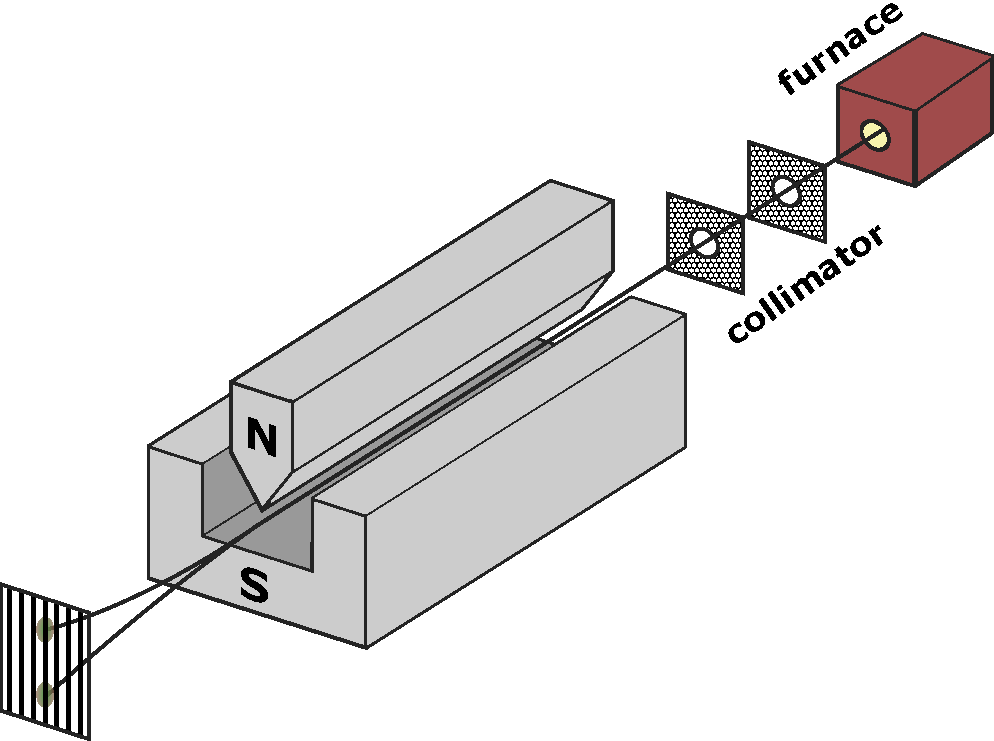
\includegraphics[width=\linewidth]{figures/stern-gerlach-setup.pdf}
  \caption{Stern-Gerlach experiment setup.}
  \label{fig:stern-gerlach}
\end{marginfigure}
A closer look of the magnetic field can be observed in fig. \ref{fig:mag-profile}.
\begin{marginfigure}%
  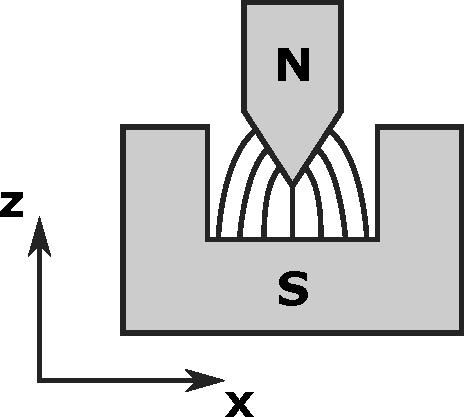
\includegraphics[width=\linewidth]{figures/field-profile.pdf}
  \caption{magnetic field profile in the Stern-Gerlach experiment setup.}
  \label{fig:mag-profile}
\end{marginfigure}
The Ag atoms carry 47 electrons, with 46 out of them being paired and the last one unpaired in the s-orbital. Thus, the magnetic moment is equal to 1$\mu_B$; in a fairly heavy atom. The classical trajectory is applicable here due to the high mass of the atom and the magnetic properties can be attributed almost exclusively to the electrons; while the magnetic moment of the nucleus is not zero, it is several orders of magnitude heavier than the electron.
Classically, the the magnetic moment was expected in a continuous spectra of values and therefore, the screen should have shown a continuous and spread distribution. However, as it is often the case in quantum mechanical systems, the outcome was different; two very localized distributions where found in the upper and lower zones as shown in fig. \ref{fig:stern-gerlach}.

The magnetic moment of the atom $\left|\vec{m}\right|$ is proportional to the electron's spin $\left|\vec{s}\right|=\pm\frac{\hbar}{2}$. The proportionality constant is $\frac{e}{m_ec}$, 

\begin{align}\label{eq:magmom}
  \left|\vec{m}\right| = \frac{e}{m_ec}\frac{\hbar}{2} = 1\mu_B.
\end{align}

The interaction energy of a dipole in a magnetic field is given by
\begin{align}\label{eq:maginteraction}
  \Delta E = -\vec{m}\vec{B},
\end{align}
and the force calculated from that potential energy is given by the gradient
\begin{align}\label{eq:magforce}
  \vec{F} = \vec{F_z} = \frac{\partial}{\partial z}(\vec{m}\vec{B})\approx m_z\frac{\partial B_z}{\partial z},
\end{align}

The potential energy is minimized when $\vec{m}$ aligns with the magnetic field $\vec{B}$. However, such alignment cannot occur unless a dissipative mechanism appears; in this case, there is no such mechanism. Thus, the magnetic moment is constantly precessing around the magnetic field in a way that he angle between both vectors and the energy $\Delta E$ are constant (see fig. \ref{fig:mom-precession}).
\begin{marginfigure}%
  \begin{centering}
    \begin{tikzpicture}
      \node[anchor=south west,inner sep=0] at (0,0) {  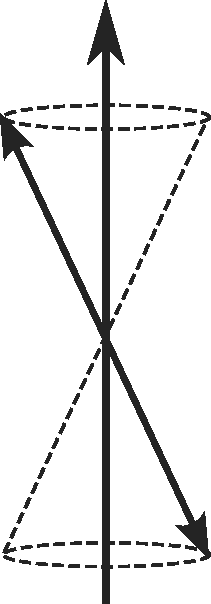
\includegraphics[width=0.3\linewidth]{figures/precessing.pdf}};
      \node at (0.75,3.1) {$\theta$};
      \node at (0.0,3.5) {$\vec{m}$};
      \node at (1.5,1.5) {$\vec{s}$};
    \end{tikzpicture}
    \caption{Magnetic moment precession around the magnetic field.}\label{fig:mom-precession}
  \end{centering}
\end{marginfigure}
In this sense, the Stern-Gerlach experiment is a device designed to measure the z-component of $\vec{m}$; giving an upwards force for $\vec{m}>0$ and a downwards force for $\vec{m}<0$. Therefore, a spread distribution of the atoms where expected according to the magnitude of their component in such direction. Conversely, two definite spots where observed (see fig. \ref{fig:s-g-results}).
\begin{marginfigure}%
  \begin{centering}
  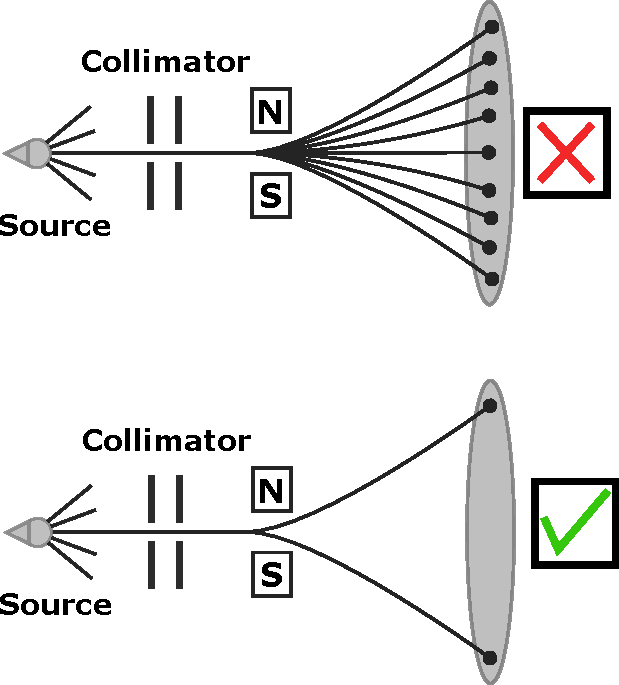
\includegraphics[width=\linewidth]{figures/s-g-result.pdf}
  \caption{Expected vs obtained result in the Stern-Gerlach experiment}
  \label{fig:s-g-results}
  \end{centering}
\end{marginfigure}
The fact that only $s_z ^+=+\frac{\hbar}{2}$ and $s_z ^-=-\frac{\hbar}{2}$ are observed but $s_z=0$ is not present, lead us to classify this momentum in a different category than the angular momentum and therefore, it stands a a magnitude of a different nature; now known as the spin momentum.

When further complexity is added to the experiment by stacking successive SG apparatuses with each stage prepared to measure a different component of the $\vec{s}$ momentum. In fig. \ref{fig:SGstack} two combination of the $s_x$ and $s_z$ measurements are shown.
\begin{marginfigure}%
  \begin{centering}
  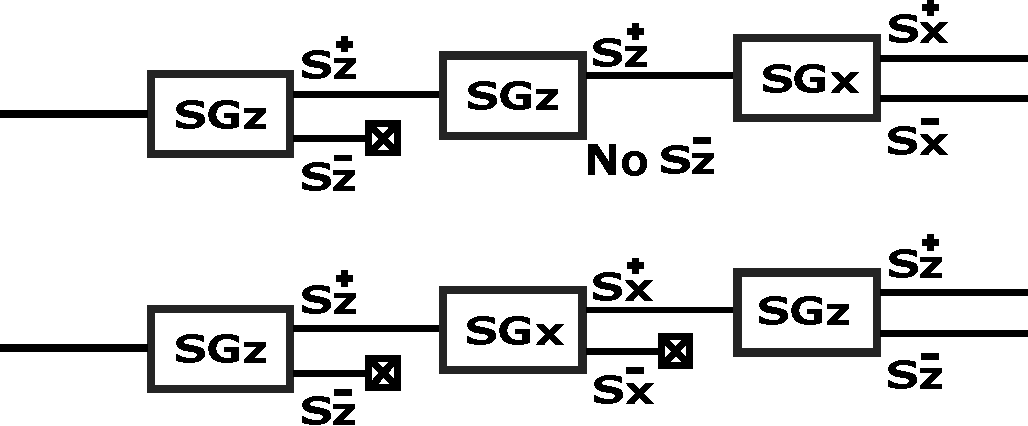
\includegraphics[width=\linewidth]{figures/SGstack.pdf}
  \caption{Stacked Stern-Gerlach experiments}
  \label{fig:SGstack}
  \end{centering}
\end{marginfigure}
In the first case, we observe a selection of the $s_z ^+$ component while the $s_z ^-$ is discarded. In the next stage, another SG apparatus in set to prove that the system is in the state $s_z ^+$ and no $s_z ^-$ is observed. In the final stage, a SGx apparatus is added; Here, due to the fact that the system is in $s_z ^+$ state, one would expect no Ag atoms passing through the experiment. The result is different than expected, obtaining the two components $s_x ^+$ and $s_x ^-$.
Here two conclusions are obtained, one is related to the destructive nature of the measuring process in quantum mechanical systems. Applying a SGz sets the system in all the possible values that $s_z$ can take; when the SGx is applied, the prior information of the system is destroyed, dividing it into the possible states $s_x$ can take. The second conclusion is that $s_z$ states are a linear superposition of $s_x$ states and vice-versa. Furthermore, it is not possible to know $s_x$, $s_y$ and $s_z$ simultaneously. Such phenomenon has no classical analogous. A classical spinning system like a top can be completely determined by its $\omega_x$, $\omega_y$, $\omega_z$ and its inertia moment I,
\begin{align}\label{eq:angularmom}
  \vec{L} = I\vec{\omega}.
\end{align}

Thus, $s_x$ and $s_z$ are defined inside an abstract two dimensional space with base vectors $\ket{s_z;+}$ and $\ket{s_z;-}$ such that
\begin{align}\label{eq:superposition}
  \ket{s_x;+}&=\frac{1}{\sqrt{2}}\ket{s_z;+}+\frac{1}{\sqrt{2}}\ket{s_z;-},\\
  \ket{s_x;-}&=-\frac{1}{\sqrt{2}}\ket{s_z;+}+\frac{1}{\sqrt{2}}\ket{s_z;-}.
\end{align}

To define the $\ket{s_y;\pm}$, we need to seek help in wave polarization phenomena. Let
\begin{align}\label{eq:monochromaticbeam}
  \vec{E}=E_0\Re\{e^{i(ky-\omega t)}\hat{e}_z\}
\end{align}
be a z-polarized monochromatic beam of light traveling in the y-direction.

\end{document}